\documentclass[10pt]{report}
\usepackage[utf8]{inputenc}
\usepackage[italian]{babel}
\usepackage{multicol}
\usepackage[bookmarks]{hyperref}
\usepackage[a4paper, total={18cm, 25cm}]{geometry}
\usepackage{graphicx}
\usepackage{xcolor}
\usepackage{textcomp}
\graphicspath{ {./img/} }
\usepackage{listings}
\usepackage{makecell}
\usepackage{qtree}
\usepackage{pgfplots}
\usepackage{tikz}
\usepgflibrary{shapes}
\usepgfplotslibrary{fillbetween}
\definecolor{backcolour}{RGB}{255,255,255}
\definecolor{codegreen}{RGB}{27,168,11}
\definecolor{codeblue}{RGB}{35,35,205}
\definecolor{codegray}{RGB}{128,128,128}
\definecolor{codepurple}{RGB}{205,35,56}
\lstdefinestyle{myPython}{
	backgroundcolor=\color{backcolour},   
	commentstyle=\color{codegreen},
	keywordstyle=\color{codeblue},
	numberstyle=\tiny\color{codegray},
	stringstyle=\color{codepurple},
	basicstyle=\small\ttfamily,
	breakatwhitespace=false,         
	breaklines=true,                 
	captionpos=b,                    
	keepspaces=true,                 
	numbers=left,                    
	numbersep=2pt,                  
	showspaces=false,                
	showstringspaces=false,
	showtabs=false,                  
	tabsize=2,
	language=python
}
\newcommand*\triangled[1]{\tikz[baseline=(char.base)]{
            \node[regular polygon, regular polygon sides=3,draw,inner sep=1pt] (char) {#1};}}
            
\usepackage{fancyhdr}
\pagestyle{fancy}
\renewcommand{\headrulewidth}{0pt}
\fancyhead{}
\fancyfoot[L]{Telegram: \texttt{@fexed}}
\fancyfoot[R]{Github: \texttt{fexed}}
\begin{document}
\title{Human Language Technologies}
\author{Federico Matteoni}
\date{A.A. 2021/22}
\renewcommand*\contentsname{Index}

\maketitle
\tableofcontents
\pagebreak
\section{Introduction}
Prof. Giuseppe Attardi\\
Prerequisites are: proficiency in Python, basic probability and statistics, calculus and linear algebra and notions of machine learning.
\paragraph{What will we learn} Understanding of and ability to use effective modern methods for \textbf{Natural Language Processing}. From traditional methods to current advanced ones like RNN, Attentions\ldots\\
Understanding the difficulties in dealing with NL and the capabilities of current technologies, with experience with \textbf{modern tools} and aiming towards the ability to build systems for some major NLP tasks: word similarities, parsing, machine translation, entity recognition, question answering, sentiment analysis, dialogue system\ldots
\paragraph{Books} Speech and Language Processing (Jurafsky, Martin), Deep Learning (Goodfellow, Bengio, Courville), Natural Language Processing in Python (Bird, Klein, Loper)
\paragraph{Exam} Project (alone or team of 2-3 people) with the aim to experiment with techniques in a realistic setting using data from competitions (Kaggle, CoNLL, SemEval, Evalita\ldots). The topic will be proposed by the team or chosen from a list of suggestions.
\paragraph{Experimental Approach}\begin{enumerate}
	\item Formulate hypothesis
	\item Implement technique
	\item Train and test
	\item Apply evaluation metric
	\item If not improved:\begin{list}{}{}
		\item Perform error analysis
		\item Revise hypothesis
	\end{list}
	\item Repeat!
\end{enumerate}
\paragraph{Motivations} Language is the most distinctive feature of human intelligence, \textbf{it shapes thought}. Emulating language capabilities is a scientific challenge, a \textbf{keystone for intelligent systems} (see: Turing test)
\paragraph{Structured vs unstructured data} The largest amount of information shared with each other is unstructured, primarily text. Information is mostly communicated by e-mails, reports, articles, conversations, media\ldots and attempts to turn text to structured (HTML) or microformat only scratched the surface.\\
Problems: requires universal agreed \textbf{ontologies} and additional effort. Entity linking attempts to provide a bridge.
\section{State of the Art}
\paragraph{Early History} During 1950s, up until AI winter.
\paragraph{Resurgence in the 1990s} Thanks to statistical methods, novelty, to study language. Challenges arise: NIST, Netflix, DARPA Grand Challenge\ldots\\
During 2010s: deep learning, neural machine translation\ldots
\paragraph{Statistical Machine Learning} Supervised training with \textbf{annotated} documents.\\
The paradigm is composed of the following:
\begin{list}{}{}
	\item Training set $\{x_i,y_y\}$
	\item Representation: choose a set of features to represent data $x\mapsto \phi(x) \in R^D$
	\item Model: choose an hypothesis function to compute $f(x) = F_\Theta(\phi(x))$
	\item Evaluation: define the cost function on error with respect to examples $J(\Theta) = \sum_i (f(x_i) - y_i)^2$
	\item Optimization: find parameters $\Theta$ that minimize $J(\Theta)$
\end{list}
It's a generic method, applicable to any problem.
\paragraph{Traditional Supervised Learning Approach} Freed us from devising algorithms and rules, requiring the creation of annotated training sets and imposing the tyranny of feature engineering.\\
Standard approach for each new problem:
\begin{list}{}{}
	\item Gather as much labeled data as one can
	\item Throw a bunch of models at it
	\item Pick the best
	\item Spend hours hand engineering some features or doing feature selection/dimensionality reduction
	\item Rinse and repeat
\end{list}
\paragraph{Technological Breakthroughs} Improved ML techniques but also large annotated datasets and more computing power, provided by GPUs and dedicated ML processors (like the TPU by Google).\\
ML exploits parallelism: stochastic gradient descent can be parallelized (asynchronous stochastic gradient descent). No need to protect shared memory access, and low (half, single) precision is enough.
\paragraph{Deep Learning Approach} Was a big breakthrough.\begin{list}{}{}
	\item Design a model architecture
	\item Define a loss function
	\item Run the network letting the parameters and the data representations \textbf{self-organize} as to minimize the loss
	\item End-to-end learning: no intermediate stages nor representation
\end{list}
\subparagraph{Feature representation} Use a vector with each entry representing a feature of the domain element\\
	Deep Learning represents data as vectors. Images are vectors (matrices), but words? \textbf{Word Embeddings}: transform a word into a vector of hundreds of dimensions capturing many subtle aspects of its meaning. Computed by the means of \textbf{language model}.\\
From a discrete to distributed representation. Words meaning are dense vectors of weights in a high dimensional space, with algebraic properties.\\
Background: philosophy, linguistics and statistics ML (feature vectors).
\subparagraph{Language Model} Statistical model which tells the probability that a word comes after a given word in a sentence.
\subparagraph{Dealing with Sentences} A sentence is a sequence of words: build a representation of a sequence from those of its words (compositional hypothesis). Sequence to sequence models.\\
Is there more structure in a sentence than a sequence of words? In many cases, tools forgets information when translating sentences into sequences of words, discarding much of the structure.
\section{Language Modeling}
\paragraph{Probabilistic Language Model} The goal is to assign a probability to a sentence.
\begin{list}{}{}
	\item \textbf{Machine Translation}: $P($high winds tonight$) > P($large winds tonight$)$
	\item \textbf{Spell Correction}: $P($about fifteen minutes from$) > P($about fifteen minuets from$)$
	\item \textbf{Speech Recognition}: $P($I saw a van$) > P($eye saw a van$)$
	\item \textbf{Language Identification}: $s$ from unknown language (italian or english) and $L$ita, $L$eng language models for italian and english $\Rightarrow$ $L$ita$(s) > L$eng$(s)$
	\item Summarization, question answering\ldots
\end{list}
We want to compute \begin{list}{}{}
	\item $P(W) = P(w_1,w_2,\ldots,w_n)$ the probability of a sequence
	\item $P(w_4\:|\:w_1,w_2,w_3,w_4)$ the probability of a word given some previous words
\end{list}
The model that computes that is called the \textbf{language model}
\paragraph{Markov Model and N-Grams} Simplify the assumption: the probability of a word given all the previous is the same of the probability of that word given just few (one, two\ldots) previous words. So $P(w_i\:|\:w_{i-},\ldots,w_1) = P(w_i\:|\:w_{i-1})$ (First order Markov chain).\\
With a \textbf{$N$-gram}: $P(w_n\:|\:w_1^{n-1}) \simeq P(w_n\:|\:w_{n-N+1}^{n-1})$\\
In general it's insufficient: language has \textbf{long distance dependencies}, but we can often get away with $N$-gram models. For example:\begin{list}{}{}
	\item “The \textbf{man} next to the large oak tree near the grocery store on the corner \textbf{is} tall.”
	\item “The \textbf{men} next to the large oak tree near the grocery store on the corner \textbf{are} tall.”
\end{list}
Or even semantic dependencies:
\begin{list}{}{}
	\item “The \textbf{bird} next to the large oak tree near the grocery store on the corner \textbf{flies} rapidly.”
	\item “The \textbf{man} next to the large oak tree near the grocery store on the corner \textbf{talks} rapidly.”
\end{list}
So more complex models are needed to handle such dependencies.
\paragraph{Maximum likelihood estimate}$$P(w_n\:|\:w_{n-N+1}^{n-1}) = \frac{\hbox{count}(w_{n-N+1}^{n-1},w_n)}{\hbox{count}(w_{n-N+1}^{n-1})}$$
Maximum because it's the one that maximize $P($Training set $|$ Model$)$
\paragraph{Shannon Visualization Method} Generate random sentences:
\begin{list}{}{}
	\item Choose a random bigram $(\langle s\rangle,w)$ according to its probability
	\item Choose a random bigram $(w,x)$ according to its probability
	\item Repeat until we pick $\langle/s\rangle$
\end{list}
\paragraph{Shannon Game} Generate random sentences by selecting the words according to the probabilities of the language models.
\begin{lstlisting}[style=myPython]
def gentext(cpd, word, length=20):
	print(word, end = ' ')
	for i in range(length):
		word = cpd[word].generate()
		print(word, end = ' ')
	print("")
\end{lstlisting}
\paragraph{Perils of Overfitting} N-grams only word well for word prediction if the test corpus looks like the training corpus. In real life, this is often not the case.\\
We need to train robust models able to adapt.
\subparagraph{Smoothing} Many rare (but not impossible) combinations of word sequences never occur in training, so MLE incorrectly assigns zero to many parameters (sparse data).\\
If a new combination occurs during testing, it is given a probability of zero and the entire sequence gets a probability of zero (infinite perplexity).\\
Parameters are \textbf{smoothed}/regularized to reassign some probability mass to unseen events (meaning removing probability from seen ones in order to maintain the joint distribution that sums to 1)
\paragraph{Zipf's Law} A small number of events occur with high frequency, while a large number of events occur with small frequency. You can quickly collect statistics on the high frequency events, but you may have to wait an arbitrarily long time to get valid statistics on low frequency events.\\
The result is that our estimates are sparse. No counts at all for the vast bulk of things we want to estimate. Some of the zeroes in the table are really zeroes, but others are simply low frequency events you haven't seen yet: after all, anything can happen. How to address? By estimating the likelihood of unseen N-grams.
\begin{center}
	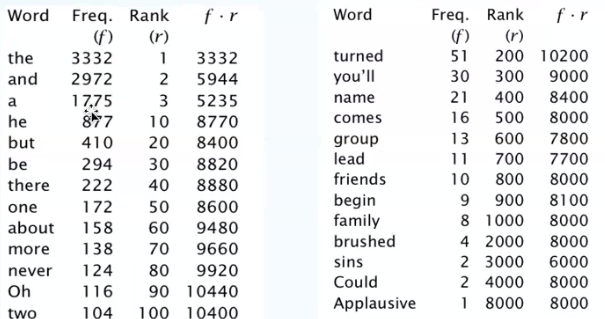
\includegraphics[scale=0.75]{1.png}
\end{center}
\textbf{Result}: $f$ is proportional to $\frac{1}{r}$, meaning that there is a constant $k\:|\:f\cdot r = k$
\begin{center}
	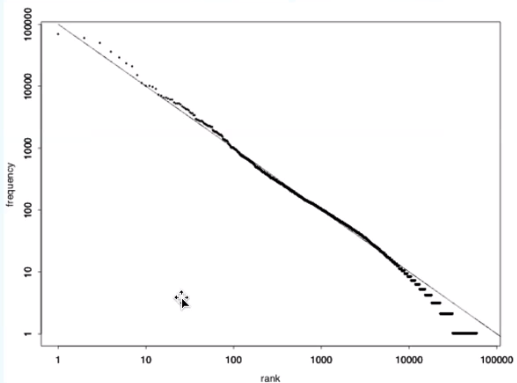
\includegraphics[scale=0.75]{2.png}
\end{center}
\subsection{Evaluation and Perplexity}
\paragraph{Evaluation} Train parameters of our model on a training set. For the evaluation, we apply the model on new data and look at the model's performance: \textbf{test set}. We need a metric which tells us how well the model is performing: one of such is \textbf{perplexity}.
\paragraph{Extrinsic Evaluation} Evaluating N-gram models.\begin{list}{}{}
	\item Put model A in a task (language identification, speech recognizer, machine translation system\ldots)
	\item Run the task, get an accuracy for $A$
	\item Put model B in the task, get accuracy for B
	\item Compare the accuracies
\end{list}
\paragraph{Language Identification Task} Build a model for each language and compute probability that text is of such language.
$$lang = arg\max_l P_l(text)$$
\paragraph{Difficulty of Extrinsic Evaluation} Extrinsic evaluation is time-consuming, can take days to run an experiment. Recent benchmarks like GLUE have become popular due to the effectiveness.\\
Intrinsic evaluation us an approximation called \textbf{perplexity}: it's a poor approximation unless the test data looks just like the training data.
\paragraph{Perplexity} The intuition is the notion of surprise: how surprised is the language model when it sees the test set? Where surprise is a measure of "I didn't see that coming". The more surprised is, the lower the probability it assigned to the test set, and the higher the probability the less surprised it is.\\
So perplexity measures how well a model "fits" the test data. It uses the probability that the model assigns to the test corpus and normalizes for the number of words in the test corpus, taking the inverse. $$PP(w) = \sqrt[N]{\frac{1}{P(w_1\ldots w_N)}}$$
Measures the weighted average branching factor in predicting the next word (lower is better).\\
In the chain rule $$PP(w) = \sqrt[N]{\prod_{i=1}^N\frac{1}{P(w_i\:|\:w_1\ldots w_{i-1})}}$$
And for bigrams $$PP(w) = \sqrt[N]{\prod_{i=1}^N\frac{1}{P(w_i\:|\:w_{i-1})}}$$
Lower perplexity $\Rightarrow$ better model
\section{Representation of Words}
\paragraph{Word Meaning} Definition of \textbf{meaning}:\begin{list}{}{}
	\item Idea represented by a word, phrase\ldots
	\item Idea that a person wants to express by using words, signs\ldots
	\item Idea expressed in a work of writing, art\ldots
\end{list}
\textbf{Signifier} (symbol) $\Leftrightarrow$ \textbf{Signified} (idea or concept) = \textbf{denotation}
\paragraph{Linguistic Solution} Dictionary or lexical resources provide word definitions as well as synonyms, hypernums, antonyms\ldots example: \textbf{Wordnet}.
\subparagraph{Problems with lexical resources} \begin{list}{}{}
	\item Imperfect, sometimes there are errors
	\item Missing new meanings of words, hard to keep up-to-date
	\item Subjective
	\item Require human labor to create and adapt
	\item Hard to compute accurate word similarity
\end{list}
\paragraph{Vector Space Model} The \textbf{VSM} is a representation for text used in information retrieval. A document is represented by a vector in a $n$-dimensional space $$v(d_1) = [t_1,\ldots, t_n]$$
Each dimension corresponds to a separate term.\\
The VSM considers words as discrete symbols.
\subparagraph{One Hot Representation} A word occurrence is represented by one-hot vectors, with the vector dimension being the number of words in a vocabulary and $1$ in correspondence of the position of the represented word. Useful for representing a document by the sum of the word occurrence vector, and document similarity given by \textbf{cosine distance} (angle between vectors).
\subparagraph{tf*idf Measure} Term frequency: frequency of the word.\\
Inverse document frequency: %TODO
\subparagraph{Classical VSM} Vector is all zeroes with $idf_t$ instead of $1$. The vector of a document is the sum of the vectors of its terms occurrence vectors.\\
Doesn't capture similarity between terms.
\paragraph{Problems with Discrete Symbols} All vectors are orthogonal, with no notion of similarity. Search engines try to address the issue using WordNet synonyms but it's better to encode the similarity in the vectors themselves.
\subparagraph{Intuition} Model the meaning of a word by "embedding" it in a vector space. The meaning of a word is a vectors of numbers (vector models are also called \textbf{embeddings}), so a \textbf{dense vector space}. Constrast: word meaning is represented in many computational %TODO
\paragraph{Word Vectors/Embeddings} Build dense vector for each word chosen so that it is similar to vectors of words that appear in similar contexts.\\
Four kinds:\begin{enumerate}
	\item[] Sparse Vector Representations
	\item Mutual-information weighted word co-occurence matrices
	\item[] Dense Vector Representations
	\item %TODO
	\item 
	\item 
\end{enumerate}
\paragraph{Distributional Hypothesis} A word's meaning is given by the words that frequently appear close-by. Old idea but successful just with modern statistical NLP.\\
When a word $w$ appears in a text, its context is the set of words that appear nearby (within a fixed-size window). Use of the many contexts of $w$ to build a representation of $w$.
\subparagraph{Word Context Matrix} Is a $|V|\times|V|$ matrix $X$ that counts the frequencies of co-occurrence of words in a collection of contexts (i.e. text spans of a given length).
\subparagraph{Co-Occurrence Matrix} Words $\equiv$ Context words. Rows of $X$ capture similarity yet $X$ is still high dimensional and sparse. One row per word with counts of occurrencies of any other word.\\
We can compute the distance vectors between words, but neighboring words are not semantically related.
\subsection{Word Embeddings}
\paragraph{Dense Representations} Project word vectors $v(t)$ into a low dimensional space $R^k$ with $k<<|V|$ of continuous space word representations (a.k.a. \textbf{embeddigns})
$$Embed : R^{|V|}\rightarrow R^k$$
$$Embed(v(t)) = e(t)$$
Desired properties: remaining dimensions %TODO
\paragraph{Collobert} Build embeddings and estimate whether the word is in the proper context using a neural network. Positive examples from text, and negative examples made replacing center word with random one. The loss for the training is $$Loss(\Theta) = \sum_{x\in X}\sum_{w\in W} \max(0, 1-f_\Theta(x) + f_\Theta(x^{(w)}))$$
with $x^{(w)}$ obtained by replacing the central word of $x$ with a random word.
\paragraph{Word2Vec} Framework for learning words, much faster to train. Idea:\begin{list}{}{}
	\item Collect a large corpus of text
	\item Every word in a fixed vocabulary is represented by a vector
	\item Go through each position $t$ in the text, which has a center word $c$ and context ("outside") words $o$
	\item Use the similarity of the word vectors for $c$ and $o$ to calculate the probability of $o$ given $c$
	\item Keep adjusting word vectors to maximize this probability
\end{list}
Two kinds:
\begin{center}
	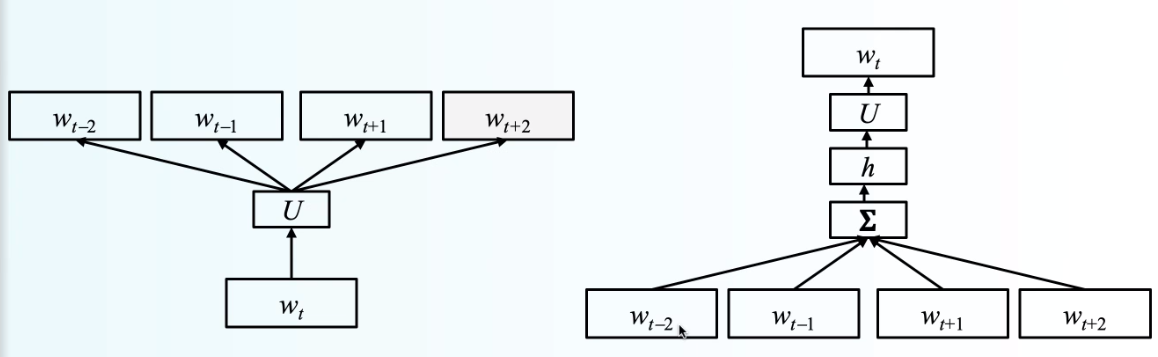
\includegraphics[scale=0.5]{3.png}
\end{center}
\begin{list}{}{}
	\item Skip-gram: predict context words within window of size $m$ given the center word $w_t$
	\begin{center}
		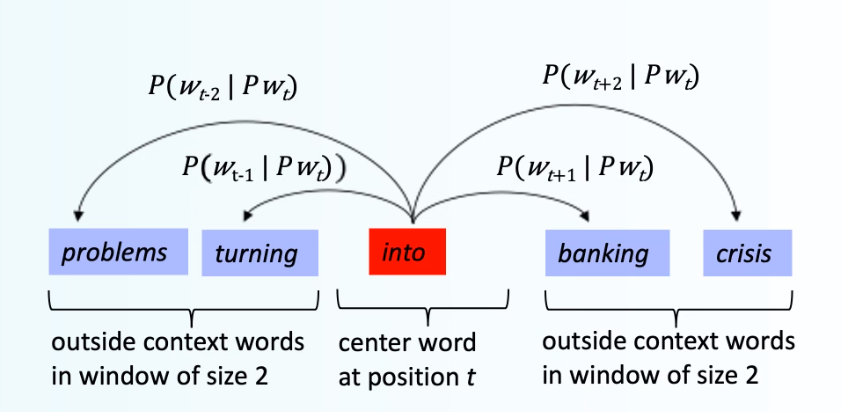
\includegraphics[scale=0.4]{4.png}
	\end{center}
	\item CBoW: predict center word $w_t$ given context words within window of size $m$
\end{list}
Embeddings are a by-product of the word prediction task. Even though it's a prediction task, the network can be trained on any text (no need for human-labeled data!).\\
Usual context size is 5 words before and after. Features can be multi-word expressions. Longer windows can capture more semantics and less syntax.\\
A typical size for $h$ is 200-300.
\subparagraph{Skip-Gram}
\begin{multicols}{2}
\begin{list}{}{}
	\item Inputs are one-hot representation of the word
	\item $w\in R^{|Vocabulary|}$ are high-dimensional
	\item $v\in R^d$ is low dimensional: size of the embedding space $d$
	\item $V\in R^{|Voc|\times d}$ input word matrix
	\item row $t$ of $V$ is the input vector, representation for \textbf{center} word $w_t$
	\item $U\in R^{d\times|Voc|}$ output matrix
	\item column $o$ of $U$ is the output vector, representation for \textbf{context} word $w_o$
\end{list}
\columnbreak
\begin{center}
	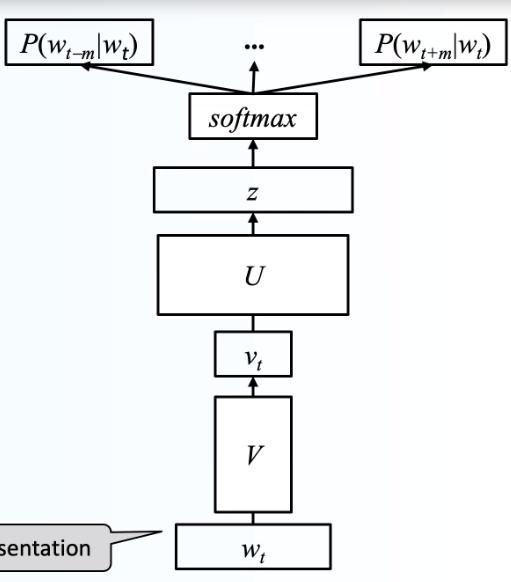
\includegraphics[scale=0.35]{5.png}
\end{center}
\end{multicols}
$v_t = w_tV$ embedding of word $w_t$\\$z=v_tU$ $z_i$ is the similarity of $w_t$ with $w_i$\\Softmax converts $z$ to a probability distribution $p_i$ $$p_i=\frac{e^{z_i}}{\sum_{j\in V}e^{z_j}}$$
Procedure
\begin{list}{}{}
	\item Lookup the embedded word vector for the center word $v_c = V[c] \in R^n$
	\item Generate score vector $z = v_cU$
	\item Turn the score vector into probabilities $\hat{y} =$ softmax$(z)$
\end{list}
$\hat{y}_{c-m},\ldots$ Those are the estimates\\ %TODO
So the training iterates through the whole corpus predicting sorrounding words given the center word.
\subparagraph{Objective Function} For each position $t=1,\ldots,T$ predict context words within a windows of fixed size $m$ given each center word $w_t$ $$\hbox{Likelihood} = L(\Theta) = \prod_{t=1}^T\prod_{-m\leq j\leq m,\:\:j\neq 0} P(w_{t+j}\:|\:w_t,\Theta)$$
While the objective function $J(\Theta)$ is the average negative log likelihood $$J(\Theta) = -\frac{1}{T}\log L(\Theta) = -\frac{1}{T}\sum_{t=1}^T\sum_{-m\leq j\leq m,\:\:j\neq 0} \log(P(w_{t+j}\:|\:w_t,\Theta)=$$
To compute $P(o\:|\:c, \Theta)$ we use two vectors per word $w$: $v_w$ when $w$ center word and $u_w$ when $w$ context word. For a center word $c$ and a context word $o$:$$P(o\:|\:c) = \frac{e^{u_o v_c}}{\sum_{w\in V} e^{u_w v_c}}$$
With the dot product $u\cdot v = \sum_i u_iv_i$: larger product $\Rightarrow$ larger probability. Normalize over entire vocabulary to give probability distribution.\\
$J(\Theta)$ is a function of all windows in the corpus, potentially billions: too expensive to compute. The solution is the stochastic gradient descent, sampling windows randomly and update after each one.
\paragraph{Softmax}\begin{list}{}{}
	\item Soft because still assign some probability to smaller $x_i$
	\item Max because amplifies the probability of largest $x_i$
\end{list}
\paragraph{Can we really capture the concept represented by a word?} Philosophical debate.
\paragraph{Negative Sampling} $\log\sum_{j\in F}e^{u_j}$ has lots of terms, costly to compute. The solution is to compute it only on a small sample of negative samples, i.e. $\log\sum_{j\in E}e^{u_j}$ where words $E$ are a few (e.g. 5) %TODO
\paragraph{CBoW} Continuous Bag of Words\\
Mirror of the skip-gram, where context words are used to predict target words.\\
$h$ is computed from the average of the embeddings of the input context, $z_i$ is the similarity of $h$ with the words embedding of $w_i$ from $U$.
\paragraph{Which Embeddings} $V$ and $U$ both define embeddigns, which to use? Usually just $V$. Sometimes average pairs of vectors from $V$ and $U$ into a single one or append one embedding vector after the other, doubling the length.
\paragraph{GloVe} Global Vectors for Word Representation. Insight: the ratio of conditional probabilities may capture meaning.
$$J = \sum_{i,j=1}^V f(X_{ij})\ldots$$
\paragraph{fastText} Similar to CBoW, word embeddings averaged to obtain good sentence representation. Pretrained models.
\paragraph{Co-Occurrence Counts}
$$P(w_t,w_{t-i},\ldots,w_{t-1}) = \frac{P(w_t,w_{t-i},\ldots,w_{t-1})}{P(w_{t-i},\ldots,w_{t-1})}$$
It's a big matrix, of $|V|\times|V|\simeq 100$k$\times100$k $\Rightarrow$ dimensionality reduction: principal component analysis, Hellinger PCA, SVD\ldots trying to reduce to size to $100$k$\times 50$, $100$k$\times 100$ or something similar, assigning each word a vector of $50$, $100$ or similar features.
\paragraph{Weighting} Weight the counts using corpus-level statistics to reflect co-occurrence significance: \textbf{Pointwise Mutual Information} $$ PMI(w_t,w_{t-i},\ldots,w_{t-1}) = \frac{P(w_t,w_{t-i},\ldots,w_{t-1})}{\log P(w_t)P(w_{t-i},\ldots,w_{t-1})} = \log\frac{\#(w_t,w_{t-i},\ldots,w_{t-1})\cdot|V|}{\#(w_{t-i},\ldots,w_{t-1})\#(w_t)}$$
Skip-gram model implicitly factorizes a shifted PMI matrix.\\
Idea of Singular Value Decomposition:
\begin{center}
	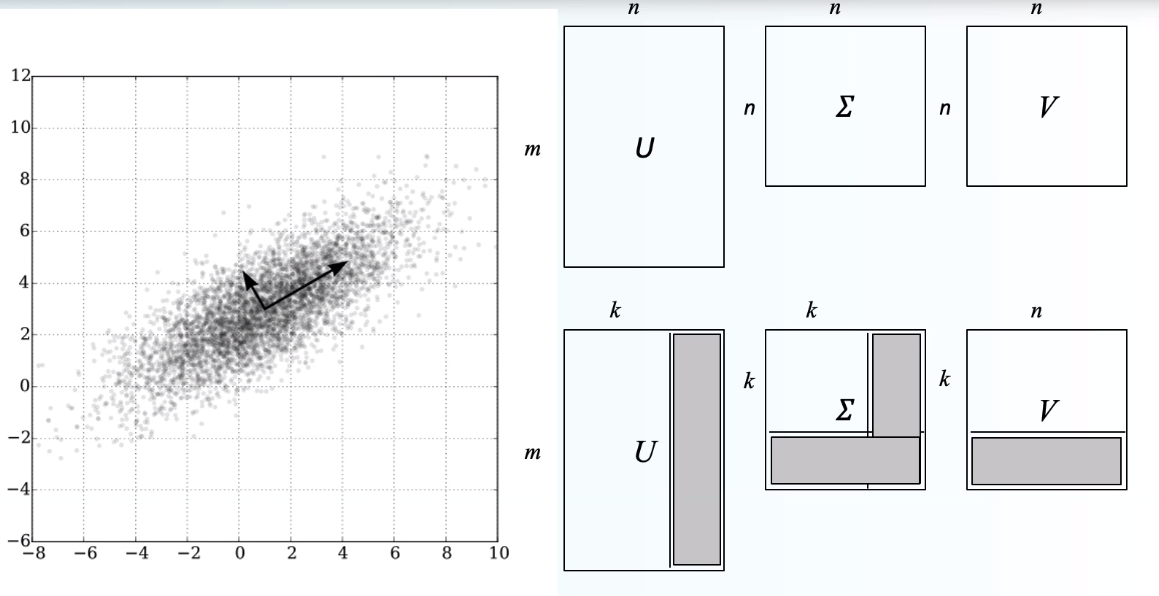
\includegraphics[scale=0.5]{6.png}
\end{center}
\subparagraph{Which One?} No clear winner. Parameters play a relevant role in the outcome of each method. Both SVD and SGNS performed well on most tasks, never underperforming significantly.\\
SGNS is suggested to be a good baseline: faster to compute and performs well.
\paragraph{Parallel word2vec} How to synchronize access to V and U, given multicore CPU to run SGD in parallel? No synchronization is good, because computation is stochastic hence it is approximate anyhow. Parameters are huge: low likelihood of concurrent access to the same memory cell. The effect is a very fast training.
\paragraph{Computing embeddings} The training cost of word2vec is linear in the size of the input. The training algorithm works well in parallel, given sparsity of words in contexts and use of negative sampling. It can be halted and restarted at anytime. %TODO
\paragraph{Gensim} Cython
\paragraph{Fang} Uses PyTorch
\subsection{Evaluation}
\paragraph{Polysemy} Word vector is a linear combination of its word senses.
$$v_{pike} = \alpha_1v_{pike_1} + \alpha_2v_{pike_3} + \alpha_3v_3$$
with $\alpha_i = \frac{f_i}{f_1+f_2+f_3}$ for the frequencies $f_i$.\\
It's intrinsic evaluation.
\paragraph{Extrinsic Vector Evaluation} The proof of the pudding is in the eating. Test on a task, e.g. NER (Named Entity Recognition)
\subsubsection{Embeddings in Neural Networks} An embedding layer is often used as fist layer in a neural network for processing text.\\
It consists of a matrix $W$ of size $|V|\times d$ where $d$ is the size of the embedding space. $W$ maps words to dense representations.\\
It is initialized either with random weights\ldots %TODO
\begin{center}
	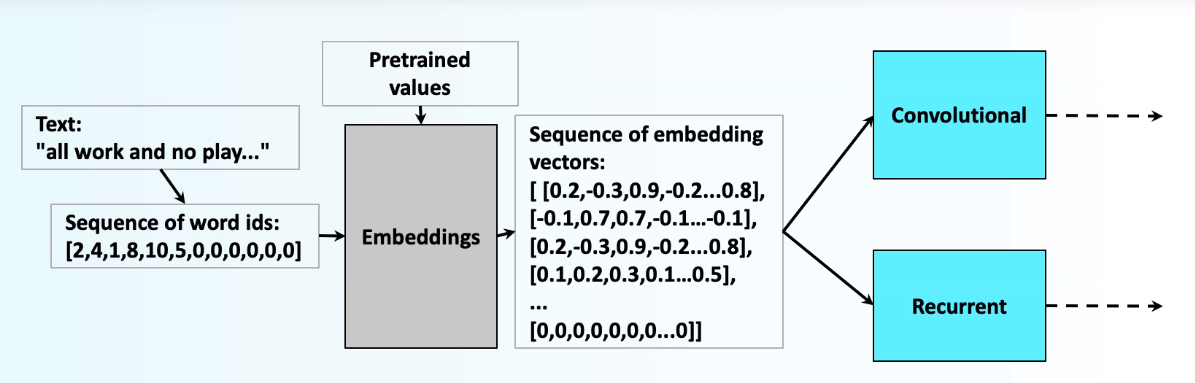
\includegraphics[scale=0.5]{7.png}
\end{center}
\subsubsection{Limits of Word Embeddings} \begin{list}{}{}
	\item Polysemous words
	\item Limited to words (neither multi words nor phrases)
	\item Represent similarity: antinomies often appear similar.\\
	Not good for sentiment analysis or polysemous words. Example:
	\begin{list}{}{}
		\item The movie was \textbf{exciting}
		\item The movie was \textbf{boring}
	\end{list}
\end{list}
\paragraph{Word Senses and Ambiguity}
\paragraph{Sentiment Specific}
\paragraph{Context Aware Word Embeddings}
\paragraph{ELMo} Embeddings from Language Model
\begin{center}
	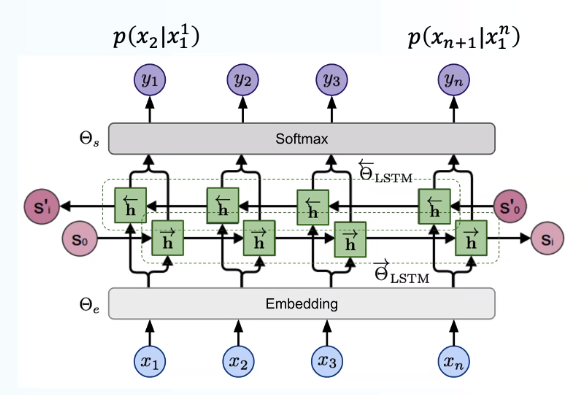
\includegraphics[scale=0.5]{8.png}
\end{center}
Given a sequence of $n$ tokens ($x_1,\ldots,x_n$) %TODO
\paragraph{OpenAI GPT-2}
\paragraph{BERT} Semi-supervised training on large amounts of text, or supervised training on a specific task with a labeled dataset.
\section{Text Classification}
For example: positive/negative review identification, author identification, spam identification, subject identification\ldots
\paragraph{Definition} The classifier $f : D \rightarrow C$ with
\begin{list}{}{}
	\item $d\in D$ input document
	\item $C=\{c_1,\ldots,c_K\}$ set of classes
	\item $c\in C$ predicted class as output
\end{list}
The learner has
\begin{list}{}{}
	\item Input: a set of $N$ hand-labeled documents $T=\{(d_1,c_1),\ldots,(d_N,c_N)\}$
	\item Output: a learned classifier $f:D\rightarrow C$
\end{list}
\begin{center}
	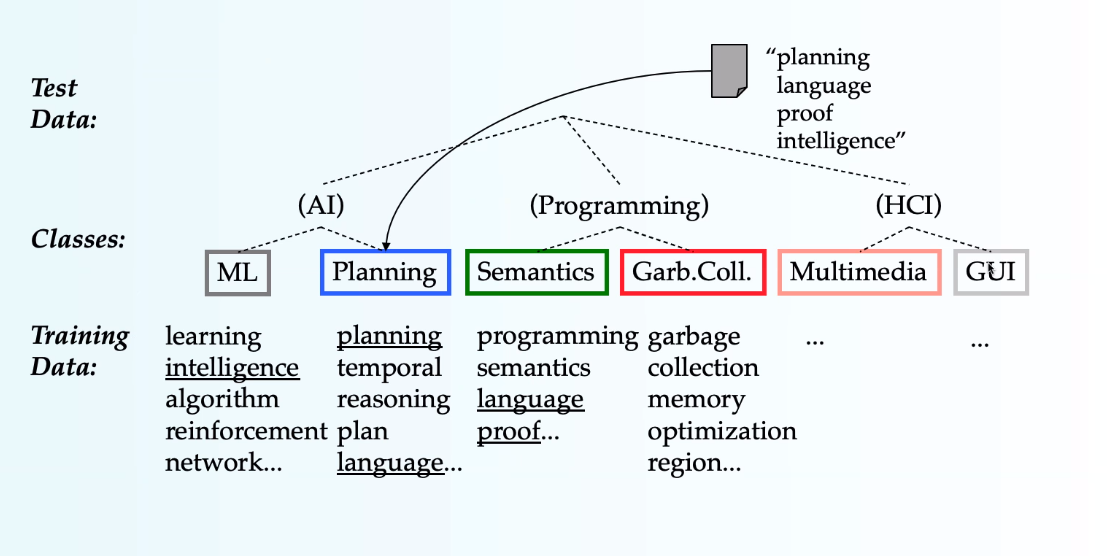
\includegraphics[scale=0.5]{9.png}
\end{center}
\paragraph{Hand-Coded Rules} Often very high accuracy, but building and maintaining these rules is expensive. For example: assign category if a document contains a given boolean combination of words (e.g. a blacklist of words for spam classification).
\paragraph{Supervised Machine Learning} Input \begin{list}{}{}
	\item A document $d\in D$
	\item A fixed set of classes $C=\{c_1,\ldots,c_K\}$
	\item A training set of $N$ hand-labeled documents $T=\{(d_1,c_1),\ldots,(d_N,c_N)\}$
\end{list}
As output\begin{list}{}{}
	\item A learned classifier $\gamma : D \rightarrow C$
\end{list}
\subsection{Naive Bayes}
A method based on the Bayes rule, relying on simple document representation (bag of words)
\paragraph{Bag of words representation} From a text, we count the frequency of each word.
\paragraph{Bayes Rule} Allows to swap the conditioning, useful because sometimes is easier estimating one kind of dependence than the other. $$P(B\:|\:A)=\frac{P(A\:|\:B)P(B)}{P(A)}$$
Applied to documents $d\in D$ and classes $c\in C$
$$P(c,d) = P(c\:|\:d)P(d) = P(d\:|\:c)P(c)$$
$$P(c\:|\:d) = \frac{P(d\:|\:c)P(c)}{P(d)}$$
\paragraph{Text classification problem} Using a supervised learning method, we want to learn a classifier $\gamma:X\rightarrow C$. The supervised learning method is denoted with $\Gamma(T)=\gamma$: it takes the training set $T$ as input and returns the learned classifier $\gamma$ that can be applied to the test set.
\subsubsection{Naive Bayes Classifiers}
We represent an instance $D$ based on some attributes $D=(x_1,\ldots, x_n)$\\Task: classify a new instance $D$ based on a tuple of attribute values into one of the calsses $c_j\in C$
$$C_{MAP}=\arg\max_{c_j\in C} P(x_1,\ldots,x_n\:|\:c_j)P(c_j)$$
\paragraph{Naive Bayes Assumption}
\begin{list}{}{}
	\item $P(c_j)$ can be estimated from the frequency of classes in the training examples
	\item $P(x_1,\ldots,x_n\:|\:c_j)$ has $O(|X|^n\cdot |C|)$ parameters and could only be estimated if a very very large number of training examples was available.
\end{list}
The \textbf{Naive Bayes Conditional Independence Assumption} is to assume that the probability of observating the conjunction of attributes is equal to the product of the individual probabilities $P(x_i\:|\:c_j)$. This means that features are independent of each other given the class
$$P(x_1,\ldots,x_n\:|\:c_j) = P(x_1\:|\:c_j)\cdot\ldots\cdot P(x_n\:|\:c_j)$$
\subsubsection{Multinomial Naive Bayes Text Classification}
$$C_B = \arg\max_{c_j\in C}P(c_j)\prod_i P(x_i\:|\:x_j)$$
Still too many possibilities. Assume the classification is independent of the position of the words, and use the same parameters for each position. The result is a \textbf{bag of words model} (over tokens, not types).
\paragraph{Learning the Model} Maximum likelihood estimate: simply use the frequencies in the data
$$\hat{P}(c_j)=\frac{\hbox{doccount}(C = c_j)}{\hbox{doccount}(T)}$$
$$\hat{P}(x_i\:|\:x_j) = \frac{\hbox{count}(X_i = x_i, C = c_j)}{\hbox{count}(C = c_j)}$$
Zero probabilities cannot be conditioned away, no matter the other evidence!
$$l = \arg\max_c \hat{P}(c)\prod_i \hat{P}(x_i\:|\:c)$$
\paragraph{Smoothing to Avoid Overfitting} For example adding 1 to the counts so that it would never be zero (\textbf{Laplace}) 
$$\hat{P}(x_i\:|\:c_j) = \frac{\hbox{count}(X_i = x_i, C = c_j) + 1}{\hbox{count}(C = c_j) + k}$$
with $k = \#$ values of $X_i$\\
Other ways: for example Bayes Unigram Prior
$$\hat{P}(x_{ik}\:|\:c_j)=\frac{\hbox{count}(X_i = x_{ik}, C = c_j) + mp_{ij}}{\hbox{count}(C = c_j) + m}$$
With $mp_{ik}$ overall fraction in data where $X_i = x_{ik}$ and $m$ extent of "smoothing".
\paragraph{Classifying} Return the most likely category for a given document$$C_{NB} = \arg\max_{c_j\in C} P(c_j)\prod_i P(w_i\:|\:c_j)$$
\paragraph{Preventing Underflow} Log space\\
Multiplying lots of prob can result in floating point underflow. It's better to perform computations by summing logs of probabilities since $\log(xy) = \log x+\log y$\\
Class with highest final unnormalized log probability is still the most probable 
$$C_{NB} = \arg\max_{c_j\in C}\log P(c_j) + \sum_i \log P(x_i\:|\:c_j)$$
Note: the model is now just a max sum of weights.
\paragraph{Generate} We can use naive bayes models to generate text, by using the probabilities of the words.
\paragraph{Naive Bayes and Language Modeling} Not the same thing, in naive we want to generalize and can use any sort of features. But if we only use word features and use all the words in a text, then Naive Bayes bears similarity to language modeling.
\paragraph{Evaluating Categorization} Must be done on data independent of the training data. Accuracy is $\frac{c}{n}$ where $n$ is the total number of test instancens and $c$ in the number of instances correctly classiefied.
\begin{center}
	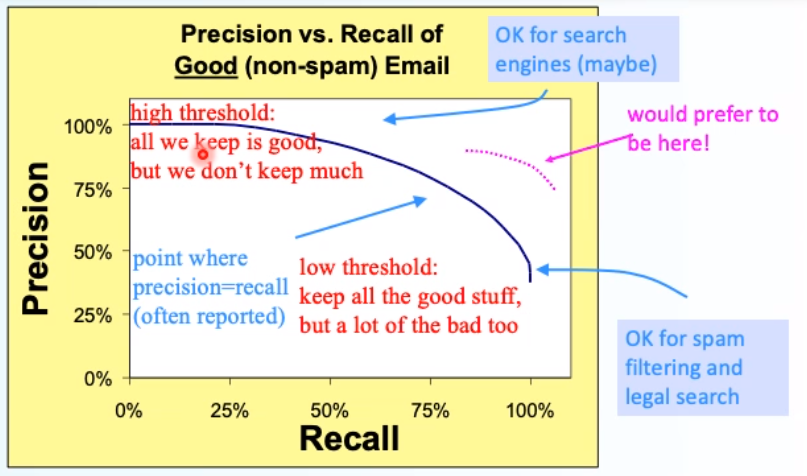
\includegraphics[scale=0.5]{10.png}
\end{center}
\begin{center}
	Contingency table\\
	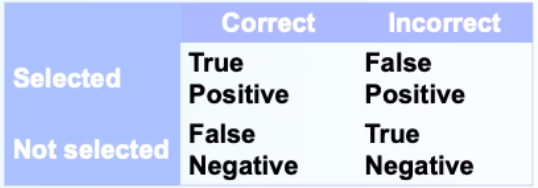
\includegraphics[scale=0.5]{11.png}
\end{center}
\paragraph{Micro vs Macro Averaging} Macro: performance for each class.\\
Micro: decision for all classes, compute contingecy table and evaluate
\paragraph{Multiclass Classification} More than 2 class, a binary classifier to dinstiguish belongin to a class and \textit{not belonging} to it.
\paragraph{Training Size} The more the better, usually.
\paragraph{Violation of Naive Bayes Assumptions} Conditional and positional independence.\\
Naive Bayss is not so naive. Among state of the art algorithms, being robust to irrelevant features (cancel each others). A good baseline for text classification, but not the best.\\
Optimal if the independence assumptions hold. Also is very fast, low storage requirements and \textbf{online learning algorithm} (incremental training, on new examples).
\paragraph{Example: SpamAssassin} Naive Bayes widely used in spam filtering.
\section{•}
\paragraph{Regular Expressions}
Formal language for specifying text strings. Letters inside square brackets, or specified ranges, like [] and [A-Z], or negations.
\paragraph{Tokenization} To do before analysis, for information retrieval and extraction, and spell-checking. Three tasks:\begin{enumerate}	
	\item Segmenting/tokenizing words in running text
	\item Normalizing word formats
	\item Segmenting sentences in running text
\end{enumerate}
\subparagraph{What's a Word?} Not easy. Babbling, in spoken language, or "are \textit{cat} and \textit{cats} the same word?".\\
Terminology:
\begin{list}{}{}
	\item \textbf{Lemma}: a set of lexical forms having the same stem, major part of speect, and rough word sense. What you would find in a dictionary.\\
	\textit{Cat} and \textit{cats} = same lemma
	\item \textbf{Wordform}: full inflected surface form.\\
	\textit{Cat} and \textit{cats} = different wordform
	\item \textbf{Type}/Form: element of the vocabulary
	\item \textbf{Token} %TODO
\end{list}
How many words? $N$ tokens and $V$ vocabulary, set of types (of size $|V|$)\\$|V|>O(N^{\frac{1}{2}})$\\
Google N-grams has $N = 1$ trillion and $|V| = 13$ million.
%TODO
\paragraph{Stanza Tokenizer} Toolkit, ternary classifier to distinguish between: normal character, end of token and end of sentence.
\paragraph{Clitics} Some languages have composite words: lascia-mi, lascia-me-lo\ldots Splitting clitics is important for parsing, since clitics incorporate relevant syntactic components (e.g. pronouns corresponding to an object of the verb).\\
Train 4-class tokenizer: normal character, end of token, end of sentence, start of clitic.
\section{Classification}
\begin{enumerate}
	\item Define classes/categories
	\item Label text
	\item Extract features
	\item Select classifier: Naive Bayes Classifiers, Decision Trees, SVMs, Neural Networks\ldots
	\item Train it
	\item Use it to classify new examples
\end{enumerate}
The data is easier to handle if it's linearly separable. Naive Bayes is slightly more general than DTs.
\paragraph{Naive Bayes} Simple model, can scale easily to millions of training examples, efficient and fast in training and classification.\\
A major limitation is the independence assumption %TODO
It's an inappropriate assumption if there are strong conditional dependencies between the variables.
\paragraph{Decision Trees} Capable to generate understandable rules, and perform classification without requiring much computation. Can handle continuous and categorical variables and provide clear indication of the important features.\\
But it's prone to errors in classification problems with many classes and small numbers of training examples. Also can be computationally expensive to train: need to compare all possible splits, and pruning can be expensive.
\paragraph{Linear vs non-linear algorithms} We find out if data is linearly or non linearly separable only empirically.\\
Linear algorithms when data is linearly separable %TODO
Non linear when data is not, more accurate but more parameters (e.g. Kernel methods)
\paragraph{Perceptron algorithm} %TODO
\subsection{Linear Binary Classification}
Data: $\{(x_i,y_i)\}$ for $i=1,\ldots,n$\begin{list}{}{}
	\item $x \in R^d$
	\item $y \in \{-1,+1\}$
\end{list}
Question: find a linear decision boundary $$wx + b$$ an hyperplane such that the classification rule associated with it has minimal probability of error.\\
Classification rule: $$y = sign(wx+b)$$
\paragraph{Perceptron} Solves if linearly separable. Basic idea: go through all existing data patterns whose label is known, if correct continue. If not, add to the weights a quantity proportional to the product of the input pattern with $y$ ($-1$ or $+1$)
\subsection{Hidden Markov Models}
\paragraph{Markov Chain} Stochastic model describing a sequence of possible events in which the probability\ldots %TODO
\begin{center}
	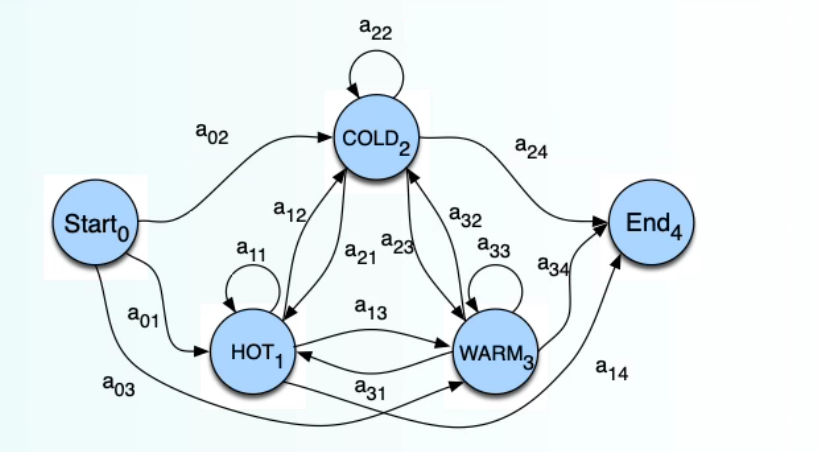
\includegraphics[scale=0.5]{12.png}
\end{center}
%salta il resto
\paragraph{Hidden Markov Model} For the chains, the output symbols are the same as the states. In named-entity of part-of-speech tagging (and speech recognition) the output symbols are \textbf{words} and the hidden states are \textbf{something else}: tags\\ %TODO
\subparagraph{Example: speech} Observed outputs are phones (speech sounds) and hidden states are phonemes (units of sound).\\
Loopbacks because a phone is circa 100ms but phones are captured every 10ms, so each phone repeats 10 times (simplifying greatly).
\begin{center}
	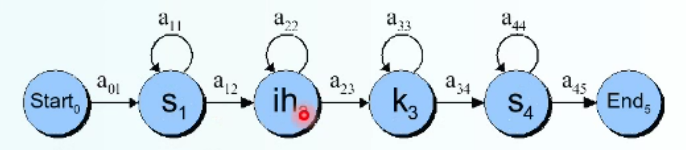
\includegraphics[scale=0.5]{14.png}
\end{center}
\begin{center}
	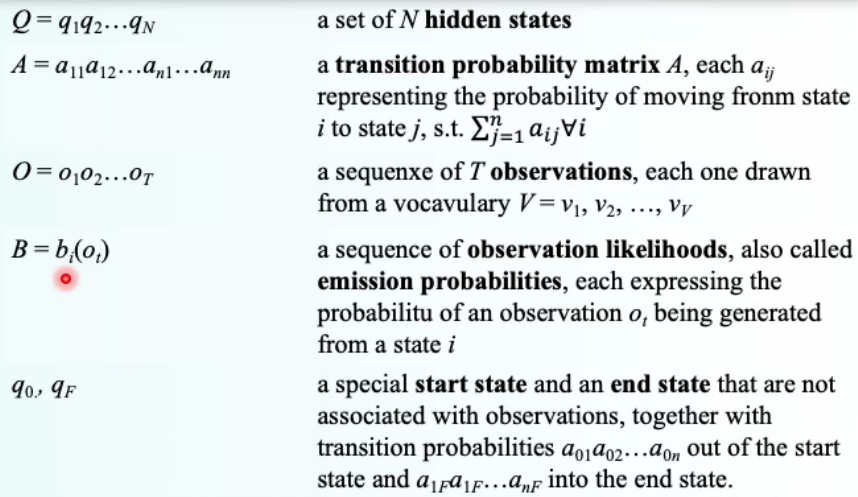
\includegraphics[scale=0.5]{13.png} %TODO riscrivere
\end{center}
\paragraph{Markov Assumption} $$P(q_i\:|\:q_1,\ldots,q_{i-1} = P(q_i\:|\:q_{i-1})$$
\paragraph{Output-independence assumption} $$P(o_t\:|\:O_1^{t-1},q_1^t)P(o_t\:|\:q_t)$$
\paragraph{Three basic problems}
\begin{list}{}{}
	\item \textbf{Evaluation}: given the observation sequence $O = (o_1,\ldots,o_T)$ and a HMM model $\Phi = (A, B)$, how to efficiently compute $P(O\:|\:\Phi)$ the probability of the observation sequence given the model?
	\item \textbf{Decoding} %TODO
	\item \textbf{Learning}: how do we adjust the model parameters $\Phi = (A,B)$ (transition and emission probabilities) to maximise $P(O\:|\:\Phi)$?
\end{list}
\paragraph{Computing the likelihood} %TODO
\begin{center}
	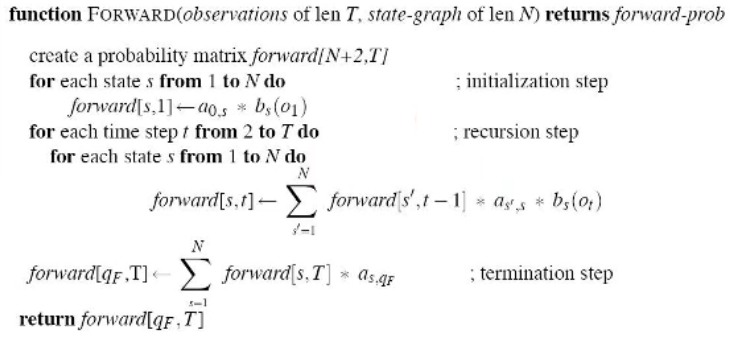
\includegraphics[scale=0.5]{15.png}
\end{center}
\paragraph{Decoding} Given an observation and a HMM, the task of the decoder is to find the best hidden state sequence.\\
Given the observation sequence $O = (o_1,\ldots,o_T)$, and a HMM $\Phi = (A, B)$, how to choose a corresponding state sequence $Q = (q_1,\ldots,q_T)$\ldots?\\ %TODO
One possibility: for each hidden state sequence $Q$, compute $P(O\:|\:Q)$ and pick the highest, but $N^T$ possibilities.\\
Instead: \textbf{Viterbi algorithm}, dynamic programming algorithm that uses similar trellis as the Forward algorithm.
\paragraph{Viterbi Algorithm} %TODO
\paragraph{Training} Baum-Welch algorithm (Expectation Maximization), no details.
\subsubsection{Part of Speech Tagging} The parts-of-speech, or lexical categories/word classes/lexical tags/POS, are nouns, verbs, adjectives, prepositions\ldots we'll use the term POS the most. Examples:
\begin{list}{}{}
	\item N, noun
	\item V, verb
	\item ADJ, adjectives
	\item ADV, adverbs
	\item \ldots
\end{list}
For example, "the koala put the keys on the table" $\rightarrow$ "DET N V\ldots"\\
But words often have more than one POS: "back" can be ADJ, ADV, N, V. POS tagging problem is determining the POS tag for a particular instance of a word.\\
We want, out of all sequences of $n$ tags $t_1,\ldots,t_n$, the single tag sequence such that $P(t_1,\ldots,t_n\:|\:w_1,\ldots,w_n)$ is the highest $$\hat{t}_1^n=\arg\max_{t_1^n} P(t_1^n\:|\: w_1^n)$$
We can compute it using the Bayes rule to transform it into a set of other probabilities that are easier to compute.
$$\hat{t}_1^n=\arg\max_{t_1^n} P(w_1^n \:|\: t_1^n)P(t_1^n)$$
Excluding the denominator because we're taking the maximum. It's composed by likelihood and prior\begin{list}{}{}
	\item Likelihood $P(w_1^n \:|\: t_1^n) \simeq \prod_{i=1}^n P(w_i\:|\:t_i)$ with the naive bayes assumption
	\item Prior $P(t_1^n)\simeq \prod$ with the markov assumption %TODO
\end{list}
\paragraph{Two kinds of probabilities}
\begin{list}{}{}
	\item Tag transition probabilities $P(t_i\:|\:t_{i-1})$ %TODO
	\item Word likelihood probabilities $P(w_i\:|\:t_i)$ %TODO
\end{list}
\subsubsection{Sequence Tagging} For example classifying each token independently using information about the surrounding tokens (sliding window) as input features.\\
For sequence tagging, sequence models work better: HMMs, MEMMs, conditional random fields, convolutional neural networks\ldots
\paragraph{Logistic Regression} Model %TODO
\paragraph{MEMM} HMM works backwards from the tags to the outputs, while MEMM works backwards: from the words to the probabilities of the tags.
\end{document}